% Consistency-Corrected Demosaicing
%
% A technical note, written to accompany src/algorithms/demosaic/
% demosaic_consistent.cpp. Not submitted anywhere.
%
% Build:  pdflatex paper.tex   (twice, for references)
%
% The tables and figures are generated by tools/paper_data.cpp so that every
% number here can be reproduced:
%   build/Release/paper_data.exe --table <raw>... > table_main.tex
%   build/Release/paper_data.exe --crops <raw> <x> <y> <size> figures/<name> <stops>

\documentclass[10pt,a4paper]{article}

\usepackage[margin=1in]{geometry}
\usepackage{amsmath}
\usepackage{amssymb}
\usepackage{graphicx}
\usepackage{booktabs}
\usepackage{subcaption}
\usepackage{url}
% algpseudocode without the `algorithm` float wrapper.
%
% `algorithm` is a FLOAT, and a float cannot break across pages. At ~90 lines
% this listing does not fit on one, so wrapping it produced a block that ran off
% the bottom of the page with stages 5 and 6 simply missing -- not overfull-box
% warnings, silently absent content.
%
% algpseudocode's own `algorithmic` environment is ordinary vertical material
% and breaks normally. The cost is losing \caption and automatic numbering,
% which for a single listing referred to by section is no loss at all.
\usepackage{algpseudocode}
\usepackage[hidelinks]{hyperref}

% \thanks rather than \footnote: inside \title, \footnote does not reliably
% typeset in the article class, whereas \thanks is the supported mechanism and
% places the note at the foot of the title page.
\title{Consistency-Corrected Demosaicing:\\
       Recovering High-Frequency Detail from Bilinear
       Reconstruction\thanks{A reference implementation, together with the
       measurement tools used to produce every figure and table in this note,
       is available at \url{https://github.com/tmeekins42/tglab}.}}
\author{Tim Meekins\\\small\texttt{tmeekins42@gmail.com}}
\date{August 2026}

\begin{document}
\maketitle

\begin{abstract}
Bilinear interpolation of a Bayer color filter array is a correct low-pass
reconstruction: its error largely vanishes under downsampling. What it discards
is high-frequency detail --- but that detail is not lost, since every sensel is
an exact measurement that bilinear has averaged away. We describe a method that
recovers it. A leave-one-out residual is computed at each site by predicting
that site's own measured channel from the reconstruction at its same-color
neighbors, excluding the sample itself; the residual is diffused off the CFA
lattice with edge-aware weighting, and applied as a single multiplicative
luminance factor common to all three channels. Because the correction is a
common scale factor it preserves channel ratios exactly and is therefore
structurally incapable of introducing false color, in contrast to additive
per-channel corrections. Measured across ten frames from three camera bodies
spanning ISO~100--12800, the method recovers more high-frequency detail than
adaptive homogeneity-directed demosaicing (median $174\%$ against $150\%$ of
bilinear at base ISO) at comparable or lower chroma noise. We report the
negative results alongside the positive ones, and describe two measurement
failures that produced confidently wrong conclusions before they were caught.
\end{abstract}

\section{Introduction}

A Bayer sensor records one color channel per photosite. Demosaicing
reconstructs the two missing channels at every site, and the difficulty is
concentrated entirely in high-frequency content: in a smooth region every method
agrees, and the differences between methods are confined to edges and fine
texture.

The observation motivating this work is that bilinear interpolation is not
merely a weak method but a \emph{correct} one in a specific and useful sense.
Averaging the neighboring samples estimates the local mean well; downsample a
bilinear reconstruction and its error largely disappears. Its failure is
band-limited --- it discards detail above the sampling frequency of each
channel.

That detail, however, has been measured. Every sensel holds an exact reading of
one channel, and bilinear has smeared it across a neighborhood. This suggests
recovering the discarded detail from the samples themselves rather than
inventing it by sharpening. The distinction matters: a sharpening kernel
amplifies whatever survived the blur, including noise, with no knowledge of the
true value. The method described here is driven entirely by the sensor data.

\section{Note on authorship and tooling}

The method described here --- treating bilinear interpolation as a correct
low-pass reconstruction, recovering the discarded detail from the sensor's own
samples, and applying that correction so as to preserve hue --- originated with
the author, as did the visual assessments on which the qualitative claims rest.

A large language model was used as a collaborator throughout. Its contribution
was the implementation in C++ and HLSL, the design and coding of the
measurement tools, the literature search reported in
Section~\ref{sec:priorwork}, and the drafting of this note. Several of the
design decisions recorded here were also arrived at in that dialogue, in both
directions: the diagnosis that an isotropic correction cannot recover
lattice-sampled detail is one; the identification of the negative-channel
mechanism in Section~\ref{sec:inject} is another; and the observation
that the sampled channel is exact, which bounds what the consistency constraint
can yield at all, came from the author.

This is disclosed for two reasons. The first is ordinary honesty about
provenance. The second is more specific to the content:
Section~\ref{sec:failures} reports two
measurement failures in which a plausible quantitative result contradicted the
rendered image, and in both cases the error was introduced by the model and
caught by human inspection of the pictures. A reader weighing the evidence here
should know which parts were machine-generated and are therefore subject to
that failure mode, and which rest on a photographer looking at photographs.

\section{Method}

\subsection{The consistency constraint}

Any reconstruction can be re-sampled through the CFA and compared against the
original mosaic. Where the two differ, the reconstruction is provably wrong ---
no ground truth and no assumption about scene content is required.

Applied naively this measures nothing. Every practical demosaicing method copies
the sampled channel verbatim, so consistency at the sampled sites is satisfied
by construction. The useful form is \emph{leave-one-out}: predict a site's own
channel from its neighbors while withholding the sample there. That prediction
can be wrong, and how wrong it is quantifies exactly what bilinear discarded.

Let $S(x,y)$ denote the normalized mosaic sample and $c$ the CFA color at
$(x,y)$. Let $P_c$ be the bilinear reconstruction of channel $c$. The residual is
%
\begin{equation}
\Delta(x,y) \;=\; S(x,y) \;-\;
  \tfrac{1}{4}\bigl[\,P_c(x{-}2,y) + P_c(x{+}2,y)
                    + P_c(x,y{-}2) + P_c(x,y{+}2)\,\bigr].
\label{eq:residual}
\end{equation}
%
The offsets are $\pm 2$ because the Bayer period is two: those four neighbors
are the nearest sites of the same color.

\subsection{Relation to Malvar--He--Cutler}

Equation~\ref{eq:residual} is not new. It is, term for term, the correction
used by Malvar, He and Cutler~\cite{malvar2004}, who describe the same quantity
as an estimated luminance change and add a gain-controlled portion of it to the
interpolated value. We arrived at it independently from the consistency
argument above, which is some evidence that the reasoning is sound, but it is
not a contribution.

The contribution, such as it is, lies in what follows: how the residual is
distributed, and how it is applied.

\subsection{Edge-aware diffusion}

The residual of Equation~\ref{eq:residual} is defined only at each site's own
color, and is therefore known on the CFA lattice --- at half of sites for
green and a quarter each for red and blue. Applying it directly would correct
in a phase-correlated pattern and reintroduce precisely the lattice artifact
that adaptive methods exist to remove.

The residual is therefore diffused across a $3\times3$ neighborhood, weighted
so that samples on the far side of an edge are excluded:
%
\begin{equation}
\tilde{\Delta}(x,y) \;=\;
  \frac{\sum_{j \in N} w_j\, \Delta_j}{\sum_{j \in N} w_j},
  \qquad
  w_j = \begin{cases}
    1 & j = (x,y)\\
    \tfrac{1}{2} & \lvert L_j - L_{(x,y)}\rvert \le \tau\\
    0 & \text{otherwise,}
  \end{cases}
\end{equation}
%
where $L$ is bilinear's luminance and $\tau = \tau_0 + \tau_1 L_{(x,y)}$. The
tolerance is proportional to the local level plus a floor, so that the same
test means the same thing in shadow and highlight; an absolute threshold
silently stops discriminating over most of the tonal range. Bilinear's
luminance is a suitable guide here because its \emph{edges} are correctly
located --- it is the detail that is missing, not the structure.

\subsection{Multiplicative luminance injection}
\label{sec:inject}

The corrected pixel is obtained by scaling all three channels by a single
factor:
%
\begin{equation}
\mathbf{c}' \;=\; k\,\mathbf{c},
\qquad
k \;=\; \mathrm{clamp}\!\left(\frac{L + s\,\tilde{\Delta}}{L},\; k_{\min},\; k_{\max}\right),
\label{eq:inject}
\end{equation}
%
where $s$ is a user strength and $L$ the reconstructed luminance.

Two properties follow. First, since $k$ multiplies every channel equally, the
ratios $R/G$ and $B/G$ are preserved exactly. This is constant-hue in the sense
of Freeman~\cite{freeman1988patent}, and it means the correction
\emph{cannot} introduce false color: no scaling of a triple can change which
channel dominates. An additive per-channel correction, such as
Malvar--He--Cutler's, has no such guarantee.

We note for precision that scaling preserves \emph{ratios}, not
\emph{differences}: $k$ maps $R - G$ to $k(R-G)$. Preserving differences
exactly would require a common additive offset instead. Ratio preservation is
the appropriate invariant, since an additive offset shifts hue in shadow where
one channel approaches zero and a fixed offset is a large relative change.

Second, the clamp on $k$ bounds the correction. An unbounded injection rings at
hard edges, which is the characteristic unpleasantness of sharpening and
precisely what this method exists to avoid.

Finally, the reconstruction is bounded by the range of real samples of the same
color in the $3\times3$ neighborhood. This is necessary rather than
defensive: camera color matrices have large negative off-diagonal terms --- a
Canon EOS~R5's first row is $[1.535, -0.555, 0.019]$ --- so a channel that is
merely \emph{short} relative to green becomes negative after the matrix, clamps
at zero, and renders fully saturated.

\subsection{Chroma median}

A $3\times3$ median is applied to the color differences $R-G$ and $B-G$,
gated on luminance similarity by the same rule as the diffusion step. Filtering
the differences rather than the channels leaves luminance detail --- the object
of the entire method --- untouched.

Median filtering of color differences after demosaicing is long-established
practice, introduced by Freeman~\cite{freeman1988patent} and exposed by dcraw
as its \texttt{-m} option. Its inclusion here is not a contribution; its
absence, however, was the one axis on which the method initially underperformed
(Section~\ref{sec:results}).

\subsection{Reduction to bilinear}

At $s = 0$ with the median disabled, Equation~\ref{eq:inject} gives $k = 1$ and
the method reduces exactly to bilinear. This is enforced by a regression test
and is what makes the measurements below trustworthy: any divergence at zero
strength is a defect in the correction rather than a property of it.

\section{Experimental method}

\subsection{Why a single error figure is inadequate}

The natural evaluation --- mean squared error against a reference --- is
actively misleading for this problem, and we report two measurements instead.

Squared error rewards not being wrong; it does not reward being sharp. A smooth
reconstruction scores well by declining to commit, and on fur, feathers and
foliage a slightly misplaced strand reads better to a human observer than a
correctly averaged smudge. This is not a rationalisation after an unfavorable
result: it is visible in the data, since the method described here scores worse
than AHD on squared error against a downsampled reference while producing
demonstrably more high-frequency energy.

A second difficulty is that any reference derived by downsampling a demosaiced
frame has already destroyed sub-pixel content --- a specular glint on a dew
drop, occupying one or two sensels --- which a method that preserves such
content is then penalised for reproducing.

We therefore measure two quantities separately:

\begin{description}
\item[Detail] the median Laplacian magnitude, normalized by local level, in
  \emph{textured} regions (local range $\ge 60\%$ of the local mean).
\item[Noise] the median local standard deviation, luminance and chroma
  separately, in \emph{flat} regions (local range $\le 25\%$ of the local mean),
  where any high-frequency content is noise by definition.
\end{description}

Both thresholds are relative to the local level so that they mean the same
thing across the tonal range. All figures are reported as a percentage of
bilinear on the same frame, which removes scene content as a variable.

\subsection{Data}

Ten raw frames from three camera bodies (Canon EOS~R5, Canon EOS~5D~Mark~III,
Sony), spanning ISO~100 to ISO~12800, covering portraiture, foliage,
architecture and backlit fine structure.

\section{Results}
\label{sec:results}

\subsection{Quantitative}

Table~\ref{tab:main} reports detail and noise for all four methods, each
relative to bilinear on the same frame.

\begin{table}[htbp]
\centering
\small
\caption{Detail and noise relative to bilinear ($=100$) on the same frame.
Detail: higher is better. Noise: lower is better. The best entry in each
column group is set in bold; bilinear is excluded from that comparison, since
it is $100$ everywhere by construction as the baseline the other figures are
expressed against. Ties are bolded jointly.}
\label{tab:main}
\begin{tabular}{lr rrr rrr rrr rrr}
\toprule
& & \multicolumn{3}{c}{Bilinear} & \multicolumn{3}{c}{Malvar}
  & \multicolumn{3}{c}{AHD} & \multicolumn{3}{c}{Proposed} \\
\cmidrule(lr){3-5}\cmidrule(lr){6-8}\cmidrule(lr){9-11}\cmidrule(lr){12-14}
Frame & ISO & Det & Lum & Chr & Det & Lum & Chr & Det & Lum & Chr
      & Det & Lum & Chr \\
\midrule
% Generated by tools/paper_data.cpp --table
% Each figure is relative to bilinear on the same frame.
\_U0A1067.CR3 & 4000 & 100 & 100 & 100 & 148 & 102 & 89 & 147 & \textbf{101} & 77 & \textbf{157} & 102 & \textbf{73} \\
\_U0A3431.CR3 & 12800 & 100 & 100 & 100 & 145 & 102 & 102 & 144 & \textbf{100} & 90 & \textbf{148} & 102 & \textbf{74} \\
\_U0A3636.CR3 & 3200 & 100 & 100 & 100 & \textbf{173} & \textbf{102} & 88 & 163 & \textbf{102} & 76 & 163 & 109 & \textbf{70} \\
\_U0A5083.CR3 & 100 & 100 & 100 & 100 & 150 & 104 & 87 & 157 & \textbf{102} & 74 & \textbf{191} & 111 & \textbf{72} \\
\_U0A6675.CR3 & 3200 & 100 & 100 & 100 & 158 & 103 & 89 & 157 & \textbf{102} & 77 & \textbf{162} & 106 & \textbf{72} \\
\_U0A6757.CR3 & 4000 & 100 & 100 & 100 & \textbf{172} & 102 & 88 & 167 & \textbf{101} & 76 & 170 & 108 & \textbf{66} \\
\_U0A6810.CR3 & 100 & 100 & 100 & 100 & 145 & 103 & 88 & 150 & \textbf{102} & 74 & \textbf{174} & 106 & \textbf{72} \\
\_MG\_9673.CR2 & 1000 & 100 & 100 & 100 & \textbf{178} & 127 & 89 & 172 & \textbf{125} & 76 & 169 & 152 & \textbf{71} \\
\_DSC0017.ARW & 125 & 100 & 100 & 100 & 168 & 105 & 90 & \textbf{175} & \textbf{103} & 79 & \textbf{175} & 117 & \textbf{75} \\
\_DSC0162.ARW & 125 & 100 & 100 & 100 & 184 & 106 & 89 & 204 & \textbf{105} & 77 & \textbf{234} & 122 & \textbf{74} \\

\bottomrule
\end{tabular}
\end{table}

The proposed method recovers the most detail on seven of ten frames and has the
lowest chroma noise on all ten. It has the lowest luminance noise on none: that
figure is consistently higher than AHD's, at $102$--$122\%$ of bilinear against
AHD's $100$--$105\%$ across nine of the ten frames, with the tenth
(\verb|_MG_9673|, $152\%$ against $125\%$) discussed below. This is the
expected consequence of restoring isolated bright samples: the method cannot
distinguish a genuine sub-pixel glint from a noise spike, and preserves both.

Two observations from the table deserve comment. The detail advantage narrows
as ISO rises ($174\%$ against AHD's $150\%$ at ISO~100; $148\%$ against $144\%$
at ISO~12800), which follows from the same mechanism: at high ISO a growing
fraction of the isolated samples being restored are noise rather than detail.
And frame \verb|_MG_9673| at ISO~1000 is an outlier in luminance noise
($152\%$), the only frame where the method's noise cost is severe; we have not
determined why.

\subsection{Qualitative}

Figures~\ref{fig:collar}, \ref{fig:hair} and~\ref{fig:fabric} show crops from a
single base-ISO portrait ($300\times300$ and $320\times320$ pixels at native
resolution), developed identically through a filmic tone curve and reproduced
without resampling.

\begin{figure}[htbp]
\centering
\begin{subfigure}{0.24\textwidth}
  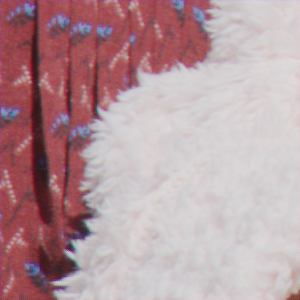
\includegraphics[width=\linewidth]{figures/collar/bilinear.png}
  \caption{Bilinear}
\end{subfigure}\hfill
\begin{subfigure}{0.24\textwidth}
  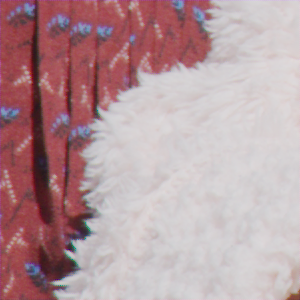
\includegraphics[width=\linewidth]{figures/collar/malvar.png}
  \caption{Malvar}
\end{subfigure}\hfill
\begin{subfigure}{0.24\textwidth}
  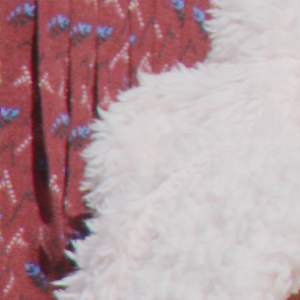
\includegraphics[width=\linewidth]{figures/collar/ahd.png}
  \caption{AHD}
\end{subfigure}\hfill
\begin{subfigure}{0.24\textwidth}
  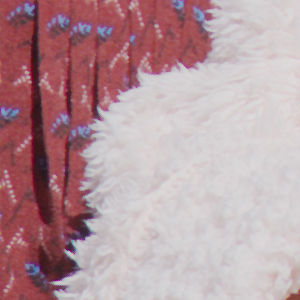
\includegraphics[width=\linewidth]{figures/collar/consistent.png}
  \caption{Proposed}
\end{subfigure}
\caption{A white fleece collar against a printed red garment: a
high-contrast, high-chroma boundary crossed by fur strands finer than the
sampling interval. Bilinear shows a cyan-green fringe along the boundary and
mottling within the printed fabric; the proposed method resolves individual
strands and leaves the boundary neutral. This is the case that motivated the
work.}
\label{fig:collar}
\end{figure}

\begin{figure}[htbp]
\centering
\begin{subfigure}{0.24\textwidth}
  
\includegraphics[width=\linewidth]{figures/hair/bilinear.png}
  \caption{Bilinear}
\end{subfigure}\hfill
\begin{subfigure}{0.24\textwidth}
  
\includegraphics[width=\linewidth]{figures/hair/malvar.png}
  \caption{Malvar}
\end{subfigure}\hfill
\begin{subfigure}{0.24\textwidth}
  
\includegraphics[width=\linewidth]{figures/hair/ahd.png}
  \caption{AHD}
\end{subfigure}\hfill
\begin{subfigure}{0.24\textwidth}
  
\includegraphics[width=\linewidth]{figures/hair/consistent.png}
  \caption{Proposed}
\end{subfigure}
\caption{Individual hair strands against a defocused background --- structures
at or below the sampling limit of the green channel. Bilinear shows pronounced
cyan and magenta speckling through the hair mass.}
\label{fig:hair}
\end{figure}

\begin{figure}[htbp]
\centering
\begin{subfigure}{0.24\textwidth}
  
\includegraphics[width=\linewidth]{figures/fabric/bilinear.png}
  \caption{Bilinear}
\end{subfigure}\hfill
\begin{subfigure}{0.24\textwidth}
  
\includegraphics[width=\linewidth]{figures/fabric/malvar.png}
  \caption{Malvar}
\end{subfigure}\hfill
\begin{subfigure}{0.24\textwidth}
  
\includegraphics[width=\linewidth]{figures/fabric/ahd.png}
  \caption{AHD}
\end{subfigure}\hfill
\begin{subfigure}{0.24\textwidth}
  
\includegraphics[width=\linewidth]{figures/fabric/consistent.png}
  \caption{Proposed}
\end{subfigure}
\caption{Printed fabric: a fine repeating pattern in saturated blue on red,
near the resolution limit. High-frequency chromatic content of this kind is
where demosaicing methods characteristically produce false color.}
\label{fig:fabric}
\end{figure}

\subsection{Cost}

At 45~megapixels on a consumer GPU the method completes in 598~ms, against
567~ms for AHD and 545~ms for Malvar. All three are bandwidth-bound rather than
compute-bound at this size, so the additional passes are nearly free.

\section{Negative results}

We report the following because they are the part of this work least likely to
exist elsewhere, and because each cost material effort.

\subsection{Consistency steering does not work}

Since the residual measures which reconstructions are wrong, it is natural to
use it to \emph{choose} an interpolation direction rather than to correct one
afterwards --- replacing AHD's least-gradient criterion with a
best-prediction criterion. This was measured before implementation, over 2.4
million decisive sites on two frames: the two criteria disagree on approximately
$45\%$ of sites, and where they disagree the gradient criterion is correct
$61$--$72\%$ of the time.

The specific case motivating the idea also failed. On textured sites, where
horizontal and vertical gradients are nearly equal and the gradient criterion
should have least information, gradient still won $56$--$63\%$. The explanation
is that smoothness of $C - G$ is not equivalent to correctness of $G$: a
systematically wrong green produces a perfectly smooth difference plane,
because the error cancels between neighbors.

\subsection{The correction saturates}

Applying more than approximately half the measured residual degrades squared
error, and full strength returns roughly to bilinear's error level. The cause
is the diffusion step: because the residual is known only on the CFA lattice,
spreading it is a blur, and that blur discards much of the high frequency the
correction exists to restore. Beyond half strength, more of a blurred
correction adds error faster than it adds detail.

The deeper limitation is that the sampled channel is exact --- every method
copies it verbatim --- so consistency at a site is free and carries no
information. The only available leverage is indirect, through channels never
measured at that site, and indirect evidence proves thin.

\section{Methodological failures}
\label{sec:failures}

Two measurement errors produced confident and wrong conclusions during this
work. Both are easy to repeat.

\paragraph{Aggregate statistics disagreed with the rendered image, in both
directions.} Removing the chroma median's edge gate improved the mean magenta
index in the dark deciles from $+0.031$ to $-0.005$, better than the reference
method --- while visibly painting green streaks along every fine strand. A
per-decile mean averages over the whole frame and cannot see a defect that is
thin, bright and localised, which was the only defect that mattered. Scoring at
edge sites, as a high percentile, and inspecting a rendered crop are all
necessary.

\paragraph{A fixture that cannot express a failure cannot test for it.} A
synthetic test scene used an identity color matrix, under which the
negative-channel mechanism of Section~\ref{sec:inject} \emph{cannot occur}. The
corresponding test passed identically with the fix present and with it removed.
Separately, a regression test for reduction to bilinear used a linear-gradient
scene, which bilinear reconstructs exactly; the residual was therefore zero and
the test could not fail regardless of how badly the strength parameter was
mishandled. Both were caught only by deliberately breaking the implementation
and confirming the test noticed.

\section{Relation to prior work}
\label{sec:priorwork}

The residual of Equation~\ref{eq:residual} is that of
Malvar--He--Cutler~\cite{malvar2004}. The chroma median postprocessing step is
Freeman's~\cite{freeman1988patent}. Neither is claimed here.

\emph{Residual Interpolation}~\cite{kiku2013,monno2017} shares terminology but
differs mechanically: its tentative estimate comes from a guided filter
regressing one channel on green, so its residual is a cross-channel model error
rather than a same-channel sampling error; it is computed without leave-one-out
exclusion, interpolated linearly rather than edge-aware, and added
per-channel rather than injected multiplicatively.

Alternating-projection methods~\cite{gunturk2002} enforce CFA consistency, but
by hard reinsertion of the known samples --- an operation that constrains the
sampled sites and does nothing to their neighbors. The diffusion step here is
what those methods lack in a single pass.

The multiplicative injection of Equation~\ref{eq:inject} is structurally the
Brovey-style detail injection used in pansharpening, where preserving band
ratios by construction is standard; the connection between CFA demosaicing and
pansharpening has been made explicitly~\cite{vivone2017}. Its nearest relative
within demosaicing is the local color ratio postprocessing of Lukac
\emph{et al.}~\cite{lukac2004}, which also preserves ratios against the
original CFA data but corrects channels sequentially through green rather than
by a single common gain.

We were unable to find this particular composition --- a Malvar-style residual,
diffused with edge awareness, injected as a common multiplicative luminance
factor --- in the literature. The honest characterisation is a novel
combination of established components rather than a new principle. The one
structural claim we would defend is that of Section~\ref{sec:inject}: the correction is
incapable of introducing false color, where an additive per-channel correction
is not.

We note also that US~7,502,505~B2 (Microsoft, filed 2004) claims computing the
gradient of Equation~\ref{eq:residual} and adding a gain-controlled portion to
an interpolated value. On a non-specialist reading its claims do not appear to
cover edge-aware diffusion or multiplicative all-channel scaling, but this
should not be relied upon.

\section{Conclusion}

Treating bilinear interpolation as a correct low-pass reconstruction, and
recovering the high-frequency content it discards from the sensor's own
measurements, produces a demosaicing method competitive with adaptive
alternatives at comparable cost. Its principal advantage is structural: because
the correction is a common multiplicative factor it cannot introduce false
color. Its principal cost is that it cannot distinguish a genuine sub-pixel
highlight from a noise spike, and consequently preserves both --- an
increasingly unfavorable trade as sensitivity rises.

\appendix

\section{Implementation}
\label{app:pseudocode}

The complete method, in the order the reference implementation performs it. All
quantities are in normalized sensor units: the mosaic sample $S$ is
$(\text{raw} - \text{black}) / (\text{white} - \text{black})$, clamped to
$[0,4]$ --- the upper bound exceeds unity because white balance is applied
after reconstruction and legitimately pushes channels above the white level.

$\mathrm{CFA}(x,y) \in \{0,1,2\}$ gives the color sampled at a site, and
$L(\mathbf{c}) = 0.2126r + 0.7152g + 0.0722b$.

% A blank line alone gives only a paragraph break, which is not enough
% separation before a listing -- the heading runs into the sentence above it.
%
% The \par before \medskip matters: vertical space placed immediately before a
% blank line is absorbed by the paragraph break that follows, so the gap below
% the heading would silently not appear. Ending the paragraph explicitly, then
% adding the skip, puts it where it is meant to go.
\bigskip
\noindent\textbf{Algorithm 1}\quad Consistency-corrected demosaicing.\par
\medskip
\begin{algorithmic}[1]
\Require mosaic $S$, strength $s$, median passes $m$
\Ensure reconstructed image $\mathbf{C}$

\Statex
\Statex \textbf{Stage 1 --- bilinear reconstruction}
\For{each site $(x,y)$}
  \State $c \gets \mathrm{CFA}(x,y)$;\quad $\mathbf{C}[c] \gets S(x,y)$
  \If{$c = 1$} \Comment{green site: the other two lie on opposite axes}
    \State $h \gets \mathrm{CFA}(x{-}1,y)$
    \State $\mathbf{C}[h] \gets \tfrac{1}{2}\bigl(S(x{-}1,y) + S(x{+}1,y)\bigr)$
    \State $\mathbf{C}[2{-}h] \gets \tfrac{1}{2}\bigl(S(x,y{-}1) + S(x,y{+}1)\bigr)$
  \Else \Comment{red or blue site}
    \State $\mathbf{C}[1] \gets \tfrac{1}{4}\bigl(S(x{\pm}1,y) + S(x,y{\pm}1)\bigr)$
    \State $\mathbf{C}[2{-}c] \gets \tfrac{1}{4}\bigl(S(x{\pm}1,y{\pm}1)\bigr)$
      \Comment{four diagonal neighbors}
  \EndIf
\EndFor

\Statex
\Statex \textbf{Stage 2 --- leave-one-out residual}
\For{each site $(x,y)$}
  \State $c \gets \mathrm{CFA}(x,y)$
  \State $p \gets \tfrac{1}{4}\bigl(\mathbf{C}_c(x{\pm}2,y) + \mathbf{C}_c(x,y{\pm}2)\bigr)$
    \Comment{this site's own sample excluded}
  \State $\Delta(x,y) \gets S(x,y) - p$
\EndFor

\Statex
\Statex \textbf{Stage 3 --- edge-aware diffusion}
\For{each site $(x,y)$}
  \State $\ell \gets L(\mathbf{C}(x,y))$;\quad $\tau \gets \tau_0 + \tau_1 \ell$
  \State $a \gets 0$;\quad $W \gets 0$
  \For{each $j$ in the $3\times3$ neighborhood}
    \If{$\lvert L(\mathbf{C}_j) - \ell \rvert \le \tau$}
      \State $w \gets 1$ if $j = (x,y)$ else $\tfrac{1}{2}$
      \State $a \gets a + w\,\Delta_j$;\quad $W \gets W + w$
    \EndIf
  \EndFor
  \If{$W > 0$} \State $\tilde{\Delta}(x,y) \gets a / W$
  \Else \State $\tilde{\Delta}(x,y) \gets 0$ \EndIf
\EndFor

\Statex
\Statex \textbf{Stage 4 --- injection and bounding}
\For{each site $(x,y)$}
  \State $\ell \gets L(\mathbf{C}(x,y))$
  \If{$\ell > \epsilon$}
    \State $k \gets \mathrm{clamp}\bigl((\ell + s\tilde{\Delta}(x,y))/\ell,\;
           k_{\min},\, k_{\max}\bigr)$
    \State $\mathbf{C}(x,y) \gets k\,\mathbf{C}(x,y)$
      \Comment{common factor: ratios preserved}
  \EndIf
  \For{$c \in \{0,1,2\}$}
    \State $[\,lo_c, hi_c\,] \gets$ range of $S$ over $3\times3$ sites
           where $\mathrm{CFA} = c$
    \State $\mathbf{C}_c \gets \mathrm{clamp}(\mathbf{C}_c,\, lo_c,\, hi_c)$
      \Comment{see \S\ref{sec:inject}}
  \EndFor
\EndFor

\Statex
\Statex \textbf{Stage 5 --- chroma median}
\State $D_r \gets \mathbf{C}_r - \mathbf{C}_g$;\quad
       $D_b \gets \mathbf{C}_b - \mathbf{C}_g$
\For{$m$ passes, and for each of $D_r$, $D_b$}
  \For{each site $(x,y)$}
    \State $V \gets \{\,D_j : j \in 3\times3,\;
           \lvert L(\mathbf{C}_j) - \ell \rvert \le \tau \,\}$
    \If{$\lvert V \rvert \ge 3$} \State $D(x,y) \gets \mathrm{median}(V)$ \EndIf
      \Comment{fewer than three is not a median}
  \EndFor
\EndFor
\State $\mathbf{C}_r \gets \mathbf{C}_g + D_r$;\quad
       $\mathbf{C}_b \gets \mathbf{C}_g + D_b$
  \Comment{green untouched: luminance detail survives}

\Statex
\Statex \textbf{Stage 6 --- color}
\State record which channels reached the clipping level, \emph{before} gains
\State $\mathbf{C} \gets \mathbf{C} \odot \text{camMul}$
\State restore clipped channels to the maximum of the three
\State $\mathbf{C} \gets M_{\text{cam}}\,\mathbf{C}$;\quad
       $\mathbf{C} \gets \max(\mathbf{C}, 0)$
\end{algorithmic}

\medskip
Constants in the reference implementation: $\tau_0 = 0.004$, $\tau_1 = 0.12$,
$k_{\min} = 0.5$, $k_{\max} = 2.0$, $\epsilon = 10^{-5}$, clipping level
$0.99$. Defaults are $s = 1$ and $m = 1$.

Two details are worth stating because they are easy to get wrong. Stage~4 must
precede stage~5: filtering the color differences before the samples have been
bounded lets the median select an out-of-range value that bounding would have
rejected, and during development this ordering error made the CPU and GPU paths
disagree by $0.008$ --- far above half-float rounding, and caught by a
cross-check rather than by eye. And stage~6's clipping decision must be taken
before the white-balance gains are applied but repaired after, since ``clipped''
is a statement about the sensor while ``neutral'' is a statement about the
balanced image.

The GPU implementation performs the same six stages as four compute kernels
over shared scratch planes, with the chroma median ping-ponging between two
pairs of planes: a pass may not read and write the same buffer, since threads
within a dispatch have no ordering.

\begin{thebibliography}{9}

\bibitem{malvar2004}
H.~S.~Malvar, L.-W.~He, and R.~Cutler,
``High-quality linear interpolation for demosaicing of Bayer-patterned color
images,''
\emph{Proc. IEEE ICASSP}, 2004.

\bibitem{freeman1988patent}
W.~T.~Freeman,
``Median filter for reconstructing missing color samples,''
U.S. Patent 4,724,395, 1988.

\bibitem{kiku2013}
D.~Kiku, Y.~Monno, M.~Tanaka, and M.~Okutomi,
``Residual interpolation for color image demosaicking,''
\emph{Proc. IEEE ICIP}, 2013.

\bibitem{monno2017}
Y.~Monno, D.~Kiku, M.~Tanaka, and M.~Okutomi,
``Adaptive residual interpolation for color and multispectral image
demosaicking,''
\emph{Sensors}, vol.~17, no.~12, 2787, 2017.

\bibitem{gunturk2002}
B.~K.~Gunturk, Y.~Altunbasak, and R.~M.~Mersereau,
``Color plane interpolation using alternating projections,''
\emph{IEEE Trans. Image Processing}, vol.~11, no.~9, pp.~997--1013, 2002.

\bibitem{lukac2004}
R.~Lukac, K.~Martin, and K.~N.~Plataniotis,
``Demosaicked image postprocessing using local color ratios,''
\emph{IEEE Trans. Circuits and Systems for Video Technology}, vol.~14, no.~6,
pp.~914--920, 2004.

\bibitem{vivone2017}
G.~Vivone \emph{et al.},
``Debayering RGBW color filter arrays: A pansharpening approach,''
2017.

\end{thebibliography}

\end{document}
